\documentclass{article}
\usepackage{amsmath}
\usepackage{amssymb}
\usepackage{graphicx}

\begin{document}

\title{Space Visualizations}
\author{Jonah Schwartzman}
\date{\today}

\maketitle

\section{Introduction}
This document is not real.

\section{Camera3D}
A Camera3D represents a viewer in 3D space, with a focal length to the view plane.
The main function of a Camera3D is to convert from a point in 3D world view to a 2D point on the view plane.
The camer3D has seven parameters:
\begin{itemize}
    \item $x$: camera x-coordinate
    \item $y$: camera y-coordinate
    \item $z$: camera z-coordinate
    \item $\theta$: pitch (angle 1)
    \item $\phi$: roll (angle 2)
    \item $\gamma$: yaw (angle 3)
    \item $f$: focal length
\end{itemize}

\section{Transform Idea}
Keep track of how the camera moves with user input, and use this to convert world points to view plane points.
\texttt{StdDraw.point(xClip, yClip)}
    \[worldPoint =  \begin{pmatrix}
    x \\ y \\ z
    \end{pmatrix}\]
    \[T(worldPoint) = \begin{pmatrix}
    \text{xClip} \\ \text{yClip}
    \end{pmatrix}\]
Find $T$ that converts from world coordinates to clipping coodinates.
\[T: WorldSpace \longrightarrow_W CameraSpace \longrightarrow_C ClipSpace\]
$C: \mathbb{R}^3 \to \mathbb{R}^2$ uses the focal length to divide out the $z$ coordinate.
So, in CameraSpace the $z$-axis is perpendicular to the view plane.
\newline\newline $W = [T]_c^w: \mathbb{R}^3 \to \mathbb{R}^3$ transforms a vector written in world coordinates to the same vector in camera coordinates.
\newline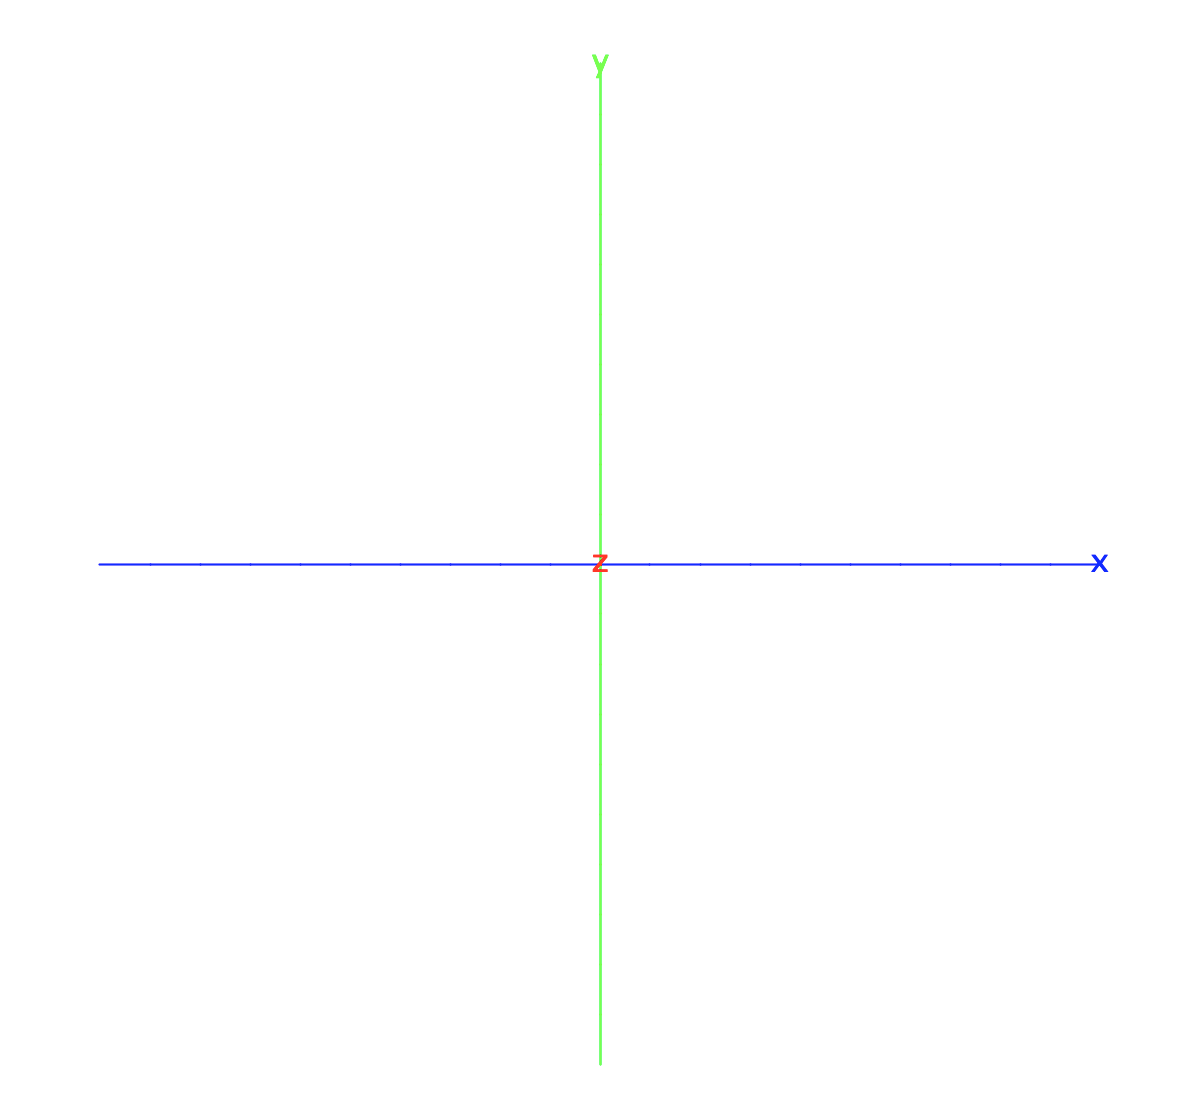
\includegraphics[scale=0.5]{3d000.png}
\newline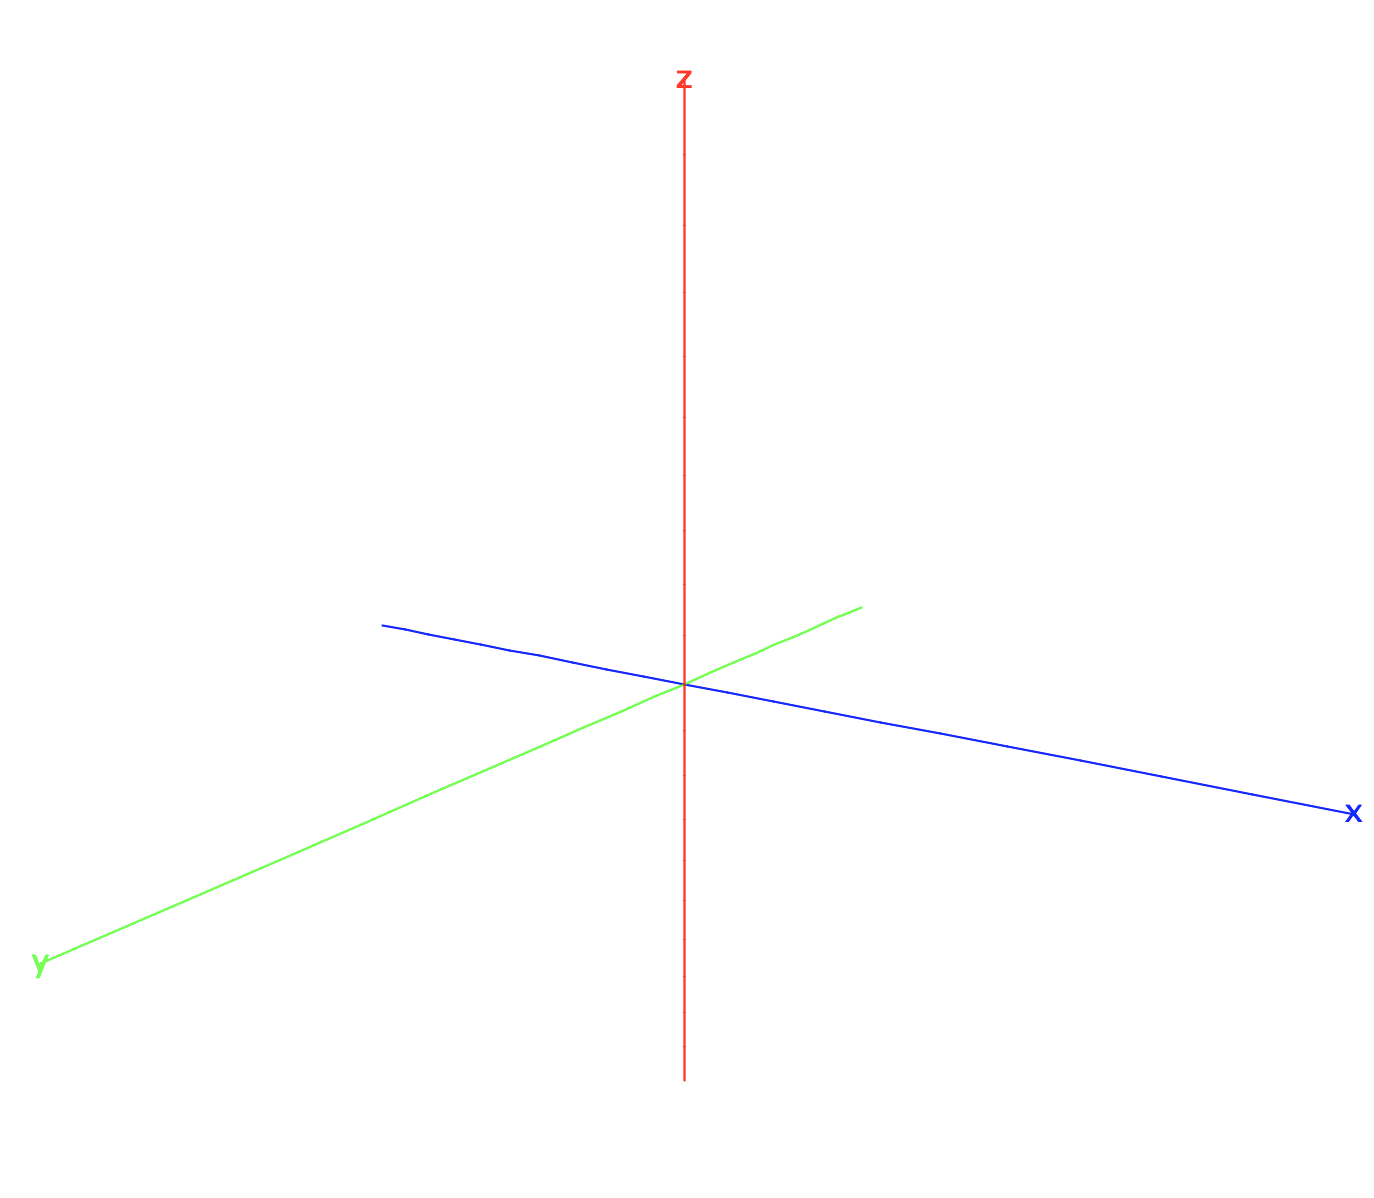
\includegraphics[scale=0.5]{3dxyz.png}

\end{document}